\documentclass[]{article}

\usepackage{tikz}
\usetikzlibrary{positioning}

% for hyperlinks and URL links
\usepackage{hyperref}

\title{\LaTeX{} Experiments\\ Part III: TikZ}

\author{AeAeA}

\begin{document}

\maketitle

%==============================================================================
\section{TikZ package}

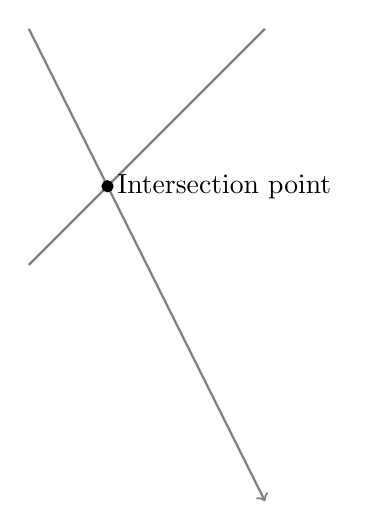
\begin{tikzpicture}
    \draw[gray, thick, ->] (-1,2) -- (2,-4);
    \draw[gray, thick] (-1,-1) -- (2,2);
    \filldraw[black] (0,0) circle (2pt) node[anchor=west] {Intersection point};
\end{tikzpicture}

\begin{itemize}
    \item \url{https://en.wikibooks.org/wiki/LaTeX/PGF/TikZ}
    \item \url{https://www.overleaf.com/learn/latex/TikZ_package}
\end{itemize}

%--------------------------------------
\subsection{Basic elements: points, lines and paths}

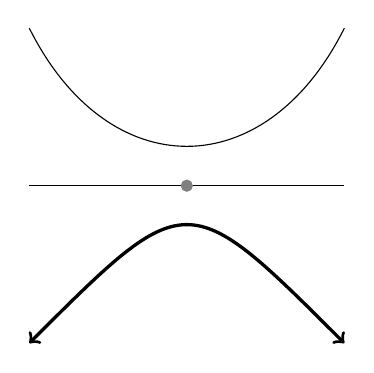
\begin{tikzpicture}
    \draw (-2,0) -- (2,0);
    \filldraw [gray] (0,0) circle (2pt);
    \draw[very thick, <->] (-2,-2) .. controls (0,0) .. (2,-2);
    \draw (-2,2) .. controls (-1,0) and (1,0) .. (2,2); 
\end{tikzpicture}

%--------------------------------------
\subsection{Basic geometric shapes: Circles, ellipses and polygons}

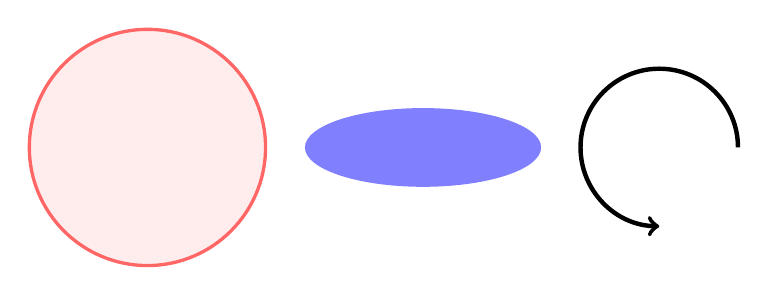
\begin{tikzpicture}
    \filldraw[color=red!60, fill=red!7, very thick] (-1,0) circle (1.5);
    \fill[blue!50] (2.5,0) ellipse (1.5 and 0.5);
    \draw[ultra thick, ->] (6.5,0) arc (0:270:1);
\end{tikzpicture}

\vspace{20pt}

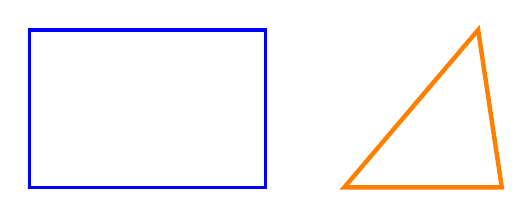
\begin{tikzpicture}
    \draw[blue, very thick] (0,0) rectangle (3,2);
    \draw[orange, ultra thick] (4,0) -- (6,0) -- (5.7,2) -- cycle;
\end{tikzpicture}

%--------------------------------------
\subsection{Diagrams with nodes}

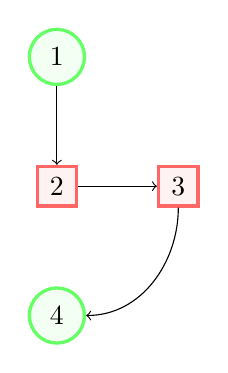
\begin{tikzpicture}[
    roundnode/.style={circle, draw=green!60, fill=green!5, very thick, minimum size=7mm},
    squarednode/.style={rectangle, draw=red!60, fill=red!5, very thick, minimum size=5mm},
    ]
    %Nodes
    \node[squarednode]      (maintopic)                              {2};
    \node[roundnode]        (uppercircle)       [above=of maintopic] {1};
    \node[squarednode]      (rightsquare)       [right=of maintopic] {3};
    \node[roundnode]        (lowercircle)       [below=of maintopic] {4};
     
    %Lines
    \draw[->] (uppercircle.south) -- (maintopic.north);
    \draw[->] (maintopic.east) -- (rightsquare.west);
    \draw[->] (rightsquare.south) .. controls +(down:7mm) and +(right:7mm) .. (lowercircle.east);
\end{tikzpicture}


\end{document}